% Template for EUSIPCO 2015 paper; to be used with:
%          spconf.sty  - LaTeX style file, and
%          IEEEbib.bst - IEEE bibliography style file.
% --------------------------------------------------------------------------
\documentclass[a4paper]{article}
\usepackage{spconf,amsmath,graphicx,cite,subfig}

% Example definitions.
% --------------------
\def\x{{\mathbf x}}
\def\L{{\cal L}}
\def\yt{\mathbf{y}_t}
\def\xt{\mathbf{x}_t}
\def\Hb{\mathbf{H}}
\def\Sb{\mathbf{S}}
\def\nt{\mathbf{n}_t}
\def\hm{\mathbf{h}_m}
\def\hathm{\hat{\mathbf{h}}_m}
\def\xtm{x_{tm}}
\def\stm{s_{tm}}
\def\Acal{\mathcal{A}}
\def\Ucal{\mathcal{U}}
\def\CN{\mathcal{CN}}

% Title.
% ------
\title{A Bayesian Nonparametric Approach for Blind Multiuser Channel Estimation}
%
% Single address.
% ---------------
%\name{Author(s) Name(s)\thanks{Thanks to XYZ agency for funding.}}
%\address{Author Affiliation(s)}
%
% For example:
% ------------
%\address{School\\
%	Department\\
%	Address}
%
% Two addresses (uncomment and modify for two-address case).
% ----------------------------------------------------------
%\twoauthors
%  {A. Author-one, B. Author-two\sthanks{Thanks to XYZ agency for funding.}}
%	{School A-B\\
%	Department A-B\\
%	Address A-B}
%  {C. Author-three, D. Author-four\sthanks{The fourth author performed the work
%	while at ...}}
%	{School C-D\\
%	Department C-D\\
%	Address C-D}
%
% Multiple author/addresses combination (use only in particular cases).
% ---------------------------------------------------------------------
\name{Isabel Valera$^*$, Francisco J. R. Ruiz$^*$, Lennart Svensson$^\dagger$, Fernando Perez-Cruz$^{*\ddagger}$ %
	%\thanks{General thanks/acknowledgment}%
	\thanks{$^*$ Isabel, Francisco and Fernando are also affiliated to the Gregorio Mara\~n´\'on Health Research Institute. Francisco J. R. Ruiz is supported by an FPU fellowship from the Spanish Ministry of Education (AP2010-5333). Isabel Valera acknowledges the support of \textit{Plan Regional-Programas I+D} of \textit{Comunidad de Madrid} (AGES-CM S2010/BMD-2422). This work is also partially supported by Ministerio de Econom\'{i}a of Spain (projects `COMONSENS', id. CSD2008-00010, and `ALCIT', id. TEC2012-38800-C03-01), by Comunidad de Madrid (project `CASI-CAM-CM', id. S2013/ICE-2845), and by the European Union 7th Framework Programme through the Marie Curie Initial Training Network `Machine Learning for Personalized Medicine' (MLPM2012, Grant No. 316861).}%
}
\address{%
    \tabular{c}
		$^*$ Universidad Carlos III de Madrid\\
		Department of Signal Processing\\and Communications\\
		Legan\'es, Spain
	\endtabular
	\hskip 0.04in
    \tabular{c}
		$^\dagger$ Chalmers University of Technology\\
		Department of Signals and Systems\\
		Gothenburg, Sweden
	\endtabular
	\hskip 0.04in
    \tabular{c}
		$^\ddagger$ Technical Staff\\at Bell Labs\\
		Alcatel-Lucent, NJ\\
	\endtabular
	\hskip 0.5in
%    \tabular{c}
%		$^\ddagger$ Bell Labs\\
%		Department GHI\\
%		Alcatel-Lucent, NJ
%	\endtabular
}

% The symbol order for multiple author combination is:
%  $^*$, $^\dagger$, $^\ddagger$, $^\mathsection$, $^\mathparagraph$, $^\|$,
%  $^{**}$, $^{\dagger\dagger}$, $^{\ddagger\ddagger}$, ...
%
%
% Alternative multiple author/addresses combination (use only in particular cases).
% ---------------------------------------------------------------------------------
%\name{A. Author-one$^*$, B. Author-two$^*$$^\dagger$, C. Author-three$^\dagger$, D. Author-four$^\ddagger$ %
%	\thanks{General thanks/acknowledgment}%
%	\thanks{$^*$ Thanks/acknowledgments for authors marked with *}%
%	\thanks{$^\dagger$ Thanks/acknowledgments for authors marked with $\dagger$}%
%	\thanks{$^\ddagger$ Thanks/acknowledgments for authors marked with $\ddagger$}%
%}
%\address{%
%	$^*$ Institute ABC, Group Group ABC, Address ABC\\
%	$^\dagger$ School DEF, Department DEF, Address DEF\\
%	$^\ddagger$ Company GHI, Department GHI, Address GHI\\
%}
%
% The symbol order for multiple author combination is:
%  $^*$, $^\dagger$, $^\ddagger$, $^\mathsection$, $^\mathparagraph$, $^\|$,
%  $^{**}$, $^{\dagger\dagger}$, $^{\ddagger\ddagger}$, ...
%
\begin{document}

%
\maketitle
%
\begin{abstract}
In many modern multiuser communication systems, users are allowed to enter and leave the system at any given time. Thus, the number of active users is an unknown and time-varying parameter, and the performance of the system depends on how accurately this parameter is estimated over time. We address the problem of blind joint channel parameter and data estimation in a multiuser communication channel in which the number of transmitters is not known. For that purpose, we develop a Bayesian nonparametric model based on the Markov Indian buffet process and an inference algorithm that makes use of slice sampling and particle Gibbs with ancestor sampling. Our experimental results show that the proposed approach can effectively recover the data-generating process for a wide range of scenarios.
\end{abstract}
%
\begin{keywords}
Bayesian nonparametric, factorial HMM, multiuser communication, machine-to-machine.
\end{keywords}
%
\section{Introduction}
\label{sec:intro}
One of the trends in wireless communication networks (WCNs) is the increase of heterogeneity. It is not new that users of WCNs are no longer only humans talking, but they also include machine-to-machine (M2M) communications, involving communication between a sensor/actuator and a corresponding application server in the network. Moreover, although there are millions of M2M cellular devices currently operating in WCNs, the industry expects this number to increase ten-fold in the years to come \cite{Dhillon2013}.
%
However, unlike consumer traffic, which is characterized by a small number of long lived sessions, the M2M traffic involves a large number of short-lived sessions with transactions of a few hundred bytes  \cite{Dhillon2013}.  
%
This results in a change of the traffic in WCNs,  leading to multiuser communication systems in which a large numbers of users may aim to enter or leave the system (i.e., start or stop transmitting) at any given time. 
%
In this context, establishing dedicated bearers for data transmission may be highly inefficient \cite{Dhillon2013}. Thus, the first question that arises is how to allow the users access the system in a way that the signaling overhead is reduced. Previous works have found that transmitting small pieces of information in the random access request itself is more efficient \cite{Chen2010}. 

In this paper, we focus on the problem of determining the number of users transmitting in a memoryless communication
system jointly with the channel estimation and the detection of the transmitted data. 
%
This problem appears in several specific applications. For instance, in the context of wireless sensor networks, where the communication nodes can often switch on and off asynchronously during operation. It also appears in massive multiple-input multiple-output (MIMO) multiuser communication systems \cite{Hoydis13}, in which the base station has a very large number of antennas and the mobile devices use a single antenna to communicate within the network. In a code-division multiple access (CDMA) context, a set of terminals randomly access the channel to communicate with a common access point, which receives the superposition of signals from the active terminals only \cite{Vazquez2013}. In the context of CDMA systems, several recent papers addressing the problem of user activity and identification can be found in the literature. The authors in \cite{AD10} propose a method to identify the number and identity of the active users in a direct sequence CDMA (DS-CDMA) system, by using a set of training data. Therefore, no symbol detection is performed in this stage.  In \cite{AD11}, a Bayesian approach, restricted to the case where the channel has been previously estimated, is presented. More recently, in \cite{Vazquez2013}, the authors solve the user identification problem while performing joint channel estimation and
data detection. 
%
A characteristic shared by all these methods is the assumption of an explicit upper bound for the number of transmitters, which makes sense in a DS-CDMA system but may represent a limitation in other scenarios.


In this paper, we propose a Bayesian nonparametric (BNP) model which, due to its nonparametric nature, becomes flexible enough to account for any number of transmitters, without the need of additional previous knowledge or bounds. Moreover, the proposed model allows us to solve this problem in a fully unsupervised way, without requiring signaling data. 
%
In particular, we assume a potentially infinite number of transmitters that might start transmitting short bursts of symbols at any time, such that only a finite subset of the transmitters become active during an observation period while the remaining (infinite) transmitters remain in an idle state (i.e., they do not transmit). 
%
Our approach consists in modeling all transmitters as an unbounded number of independent chains in an infinite factorial hidden Markov model (iFHMM) \cite{IFHMM}, in which each chain representing a transmitter has high probability of remaining in its current state (either active or idle). Under this model, the symbols sent by each transmitter can be viewed as a hidden sequence that the receiver needs to reconstruct from the observations (i.e., the received sequence). 
%Due to its nonparametric nature, our model becomes flexible enough to account for any number of transmitters, without the need of additional previous knowledge or bounds. 
%
Our experimental results show that the proposed approach efficiently  solves user identification, channel estimation and
data detection in a jointly and fully blind way and, as a consequence, they shed light on the suitability of BNPs applied to signal processing for communications.


%constitutes one of the first steps in the research on the application of BNP approaches to signal processing for communications.

%shed light on future research for the application of BNP approaches to signal processing for communications.

% \footnote{Note that the IFHMM in \cite{IFHMM} defines a probability distribution over an unbounded number of binary Markov chains (i.e., it allows only the active and inactive states). Then, we need to extend this model to account for any number of states, which will include the symbols sent by each transmitter while active.}


\section{Proposed System Model}
\label{sec:approach}

Let us assume a multiuser digital memoryless communication system with $M$ transmitters (users) and $R$ receiving antennas. Each receiving antenna observes a linear combination of all the transmitted data sequences, corrupted by additive white Gaussian noise (AWGN).\footnote{Our model is also applicable for non-Gaussian noise models.} Specifically, the $R$-dimensional observation vector compound of the observations at all the receiving antennas at time instant $t$ can be written as
\begin{equation}
\yt = \sum_{m=1}^{M} \hm \xtm+\nt, \label{eq:Obs_eq}
\end{equation}
where $\xtm$ is the symbol sent by transmitter $m$ at time instant $t$, $\hm$ is an $R$-vector containing the channel coefficients between the $m$-th transmitter and all the receiving antennas, and $\nt$ denotes the additive noise. Figure~\ref{fig:MIMOchannel} shows a diagram of such digital communication system, where a set of users or transmitters (`Tx') send their messages to a unique receiver (`Rx'), equipped with multiple antennas.

\begin{figure}[h]
\centering
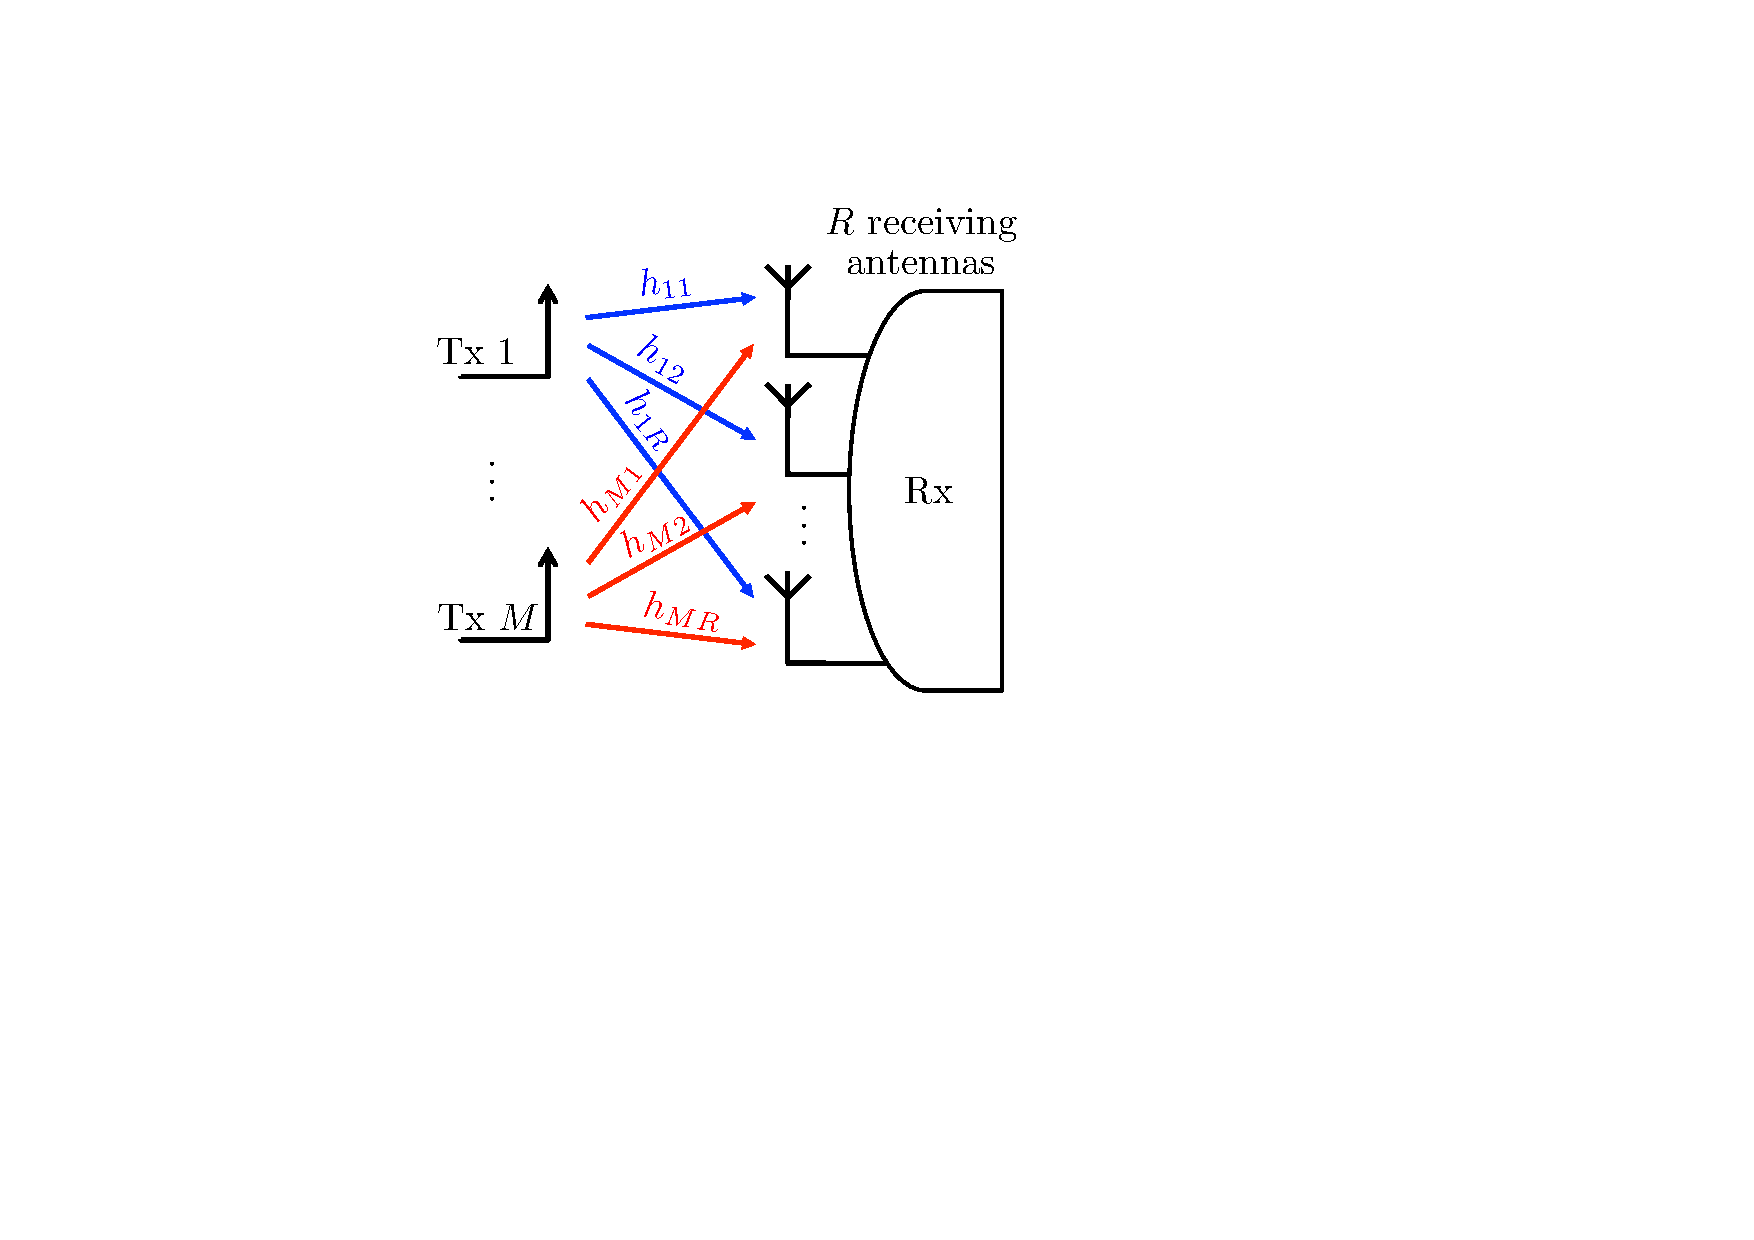
\includegraphics[width=0.21\textwidth]{figures/MIMOchannel.pdf}
\caption{Illustration of a digital communication system.}\label{fig:MIMOchannel}
\end{figure}

Transmitters are allowed to start or stop transmitting at any given time and, while active, the $m$-th transmitter sends symbols $\xtm$ that belong to a complex constellation $\Acal$, with cardinality $|\Acal|$. While idle, we can assume that $\xtm=0$ and, therefore, each symbol $\xtm\in\Acal \bigcup \{0\}$. Moreover, according to \eqref{eq:Obs_eq}, the observation $y_t$ only depends on the transmitted symbols by the active transmitters at time $t$.  Hence, we can assume an infinite number of transmitters in the system ($M\rightarrow\infty$) by ensuring that only a finite subset $M_+$ of them become active during the observation period $\{1,\ldots,T\}$, while the rest do not influence the observations.

In a realistic scenario, symbols tend to be transmitted as bursts. We model this effect with a first-order HMM that favors high self-transition probabilities of the active and inactive states. We introduce the auxiliary binary variable $\stm$ to indicate whether the $m$-th transmitter is active at time $t$, such that $\xtm=0$ if $\stm=0$ and $\xtm\sim\Ucal(\Acal)$ if $\stm=1$, being $\Ucal(\Acal)$ the uniform distribution over the set $\Acal$. We additionally introduce the variable $a_m$ to denote the self-transition probability of the inactive state for the $m$-th transmitter, such that
\begin{equation}
p(\stm=0|s_{(t-1)m}=0,a_m) = a_m,
\end{equation}
and the variable $b_m$ to denote the transition probability from active to inactive, i.e.,
\begin{equation}
p(\stm=0|s_{(t-1)m}=1,b_m) = b_m,
\end{equation}
and we assume a dummy initial state $0$ for all transmitters at time $t=0$. Figure~\ref{fig:modelSketch} shows an example of our factorial HMM.

\begin{figure}[b]
\centering
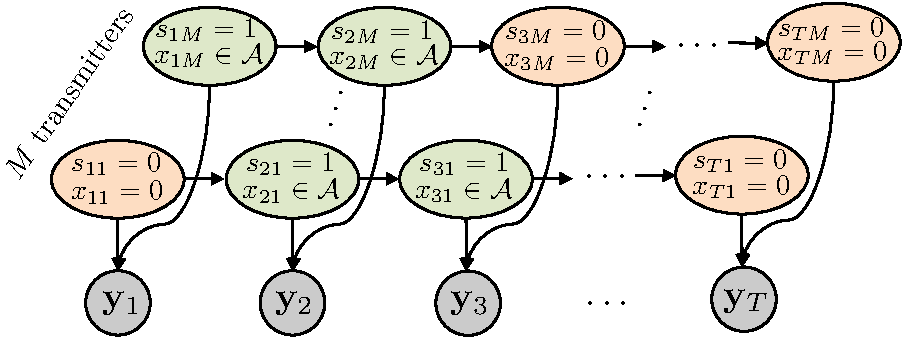
\includegraphics[width=0.45\textwidth]{figures/modelSketch.pdf}
\caption{Illustration of an example of our factorial model.}\label{fig:modelSketch}
\end{figure}

In order to complete the description of our model, we need to specify the prior distribution over all the hidden variables. To allow for an infinite number of transmitters, we rely on the iFHMM in \cite{IFHMM} and place a Markov Indian buffet process (mIBP) prior over the $T\times M$ matrix $\Sb$ that contains all variables $\stm$, i.e., $\Sb\sim \textrm{mIBP}(\alpha,\gamma_1,\gamma_2)$. The mIBP is a prior over binary matrices with an infinite number of columns (transmitters), in which each column follows an HMM. The mIBP ensures that only a finite number of the columns become active for any finite number of rows (observations) $T$. This prior distribution can also be obtained by placing the priors
\begin{equation}
a_m\sim\textrm{Beta}\left(1,\frac{\alpha}{M}\right),\quad b_m\sim\textrm{Beta}(\gamma_1,\gamma_2),
\end{equation}
and taking the limit as $M\rightarrow\infty$ \cite{IFHMM}. Regarding the hyperparameters of the model, in our experiments we set $\alpha=1$, $\gamma_1=0.1$ and $\gamma_2=2$. Note that these values of $\gamma_1$ and $\gamma_2$ favor the state persistence of the active state.

We finally place a circularly symmetric complex Gaussian prior distribution with independent elements over the channel coefficients $\hm$ and the noise $\nt$ of the form
\begin{equation}
\hm \sim \CN(\mathbf{0},\sigma_h^2 \mathbf{I}),\quad
\nt \sim \CN(\mathbf{0},\sigma_n^2 \mathbf{I}).
\end{equation}
This corresponds to a Rayleigh fading AWGN channel.

\section{Inference}
\label{sec:inference}

We now focus on the joint estimation of the number of active users, the symbols they transmit and the channel coefficients given the sequence of observations $\{\mathbf{y}_1, \ldots, \mathbf{y}_T\}$. To this end, we derive an MCMC-based algorithm which sequentially samples from the posterior probability of the unknown variables as follows:
\begin{itemize}
\item \textbf{Step 1:} Add $M_{\textrm{new}}$ new inactive transmitters. Note that at this step we restrict the considered number of transmitters in the system to $M_+ +M_{\textrm{new}}$.
\item \textbf{Step 2:} Jointly sample the states $\stm$ and the symbols $\xtm$ sent by the considered transmitters in the observation period. Remove those transmitters that remain inactive in the whole observation period (updating $M_+$).
\item \textbf{Step 3:} For each active transmitter $m=1,\ldots, M_+$, sample the transition probabilities ($a_m$ and $b_m$) and the channel coefficients $\hm$.
\end{itemize}

In \textbf{Step 1}, we make use of a slice sampling  algorithm that resorts to the stick-breaking construction of the mIBP to add a set of new inactive transmitters, sampling their self-transition probabilities of the inactive state $a_m$ \cite{StickBreakingIBP}. For these new inactive users, the probabilities $b_m$  and the channel coefficients $\hm$ are drawn from the prior.
%
\textbf{Step 2} consists in a particle Gibbs with ancestors sampling (PGAS) algorithm \cite{lindsten2014particle}. We make use of this algorithm because it allows us to jointly sample all the states $\stm$ and transmitted symbols $\xtm$ of all the considered transmitters for each time instant $t$. This leads to a significant improvement in the mixing properties of the algorithm in comparison to the forward-filtering backward-sampling in \cite{IFHMM}, which samples the sequence of states and symbols sequentially for each transmitter (and conditioning on the symbols of the remaining transmitters). Afterwards, we remove the transmitters that remain inactive during the whole observation period, consequently updating $M_+$. 
%
Finally, in \textbf{Step 3}, we sample the parameters of the active users (the transition probabilities $a_m$ and $b_m$, and the channel coefficients $\hm$) from their posterior distributions, conditioned on the observations $\yt$ and on the symbols $\xtm$.


\section{Experiments}
\label{sec:experiments}
We now run a battery of experiments to illustrate the performance of the proposed approach. To this end, we simulate different scenarios of a multiuser communication system, considering different values for the number of transmitters $M_+$, the number of receivers $R$, and the signal-to-noise ratio (SNR), which we define as $\mathrm{SNR (dB)} = -10 \log (\sigma^2_n)$. 

To generate the observations, we assume that each of the $M_+$ transmitters sends a burst of symbols during the observation period of length $T=500$. Transmitters use quadrature amplitude modulation (QAM) with cardinality $|\Acal|$, being the symbols in the constellation normalized to yield unit energy. We assume that each transmitter becomes active at a random instant, uniformly sampled in the interval $\{1, \ldots, T/2 \}$, being the burst duration sampled from a negative binomial distribution with mean $200$ and standard deviation $50$. As we described in Section~\ref{sec:approach}, the channel is assumed to be Rayleigh and AWGN, i.e., the channel coefficients and the noise are circularly symmetric complex Gaussian distributed with zero mean, being the covariances matrices $\sigma_h^2 \mathbf{I}$ and $\sigma_n^2 \mathbf{I}$, respectively. We assume $\sigma_h^2=1$, while $\sigma_n^2$ depends on the considered SNR.

%We evaluate the performance of the model in terms of detection error probability (DEP), defined as the error probability of detecting the true number of active transmitters, i.e., the probability that the inferred number of active transmitters $\hat{M}_+$ differs from the true number of active transmitters $M_+$.  Additionally,

For those cases in which the true value of the number of transmitters is recovered (i.e.,  $\hat{M}_+ =M_+$), we evaluate the performance in terms of the activity detection error rate (ADER), the symbol error rate (SER), and the mean square error (MSE) of the channel coefficient estimates. The ADER is the probability of detecting activity (inactivity) in a transmitter while that transmitter is actually inactive (active). When computing the SER, an error is computed at time $t$ whenever the estimated symbol for a transmitter differs from the actual transmitted symbol, considering that the transmitted symbol while inactive is $\xtm=0$. We can compute the MSE as
\begin{equation}
\mathrm{MSE} = \frac{1}{R M_+}  \sum_{m=0}^{M_+} \|\hm- \hathm\|^2,
\end{equation} 
where $\hathm$ is the $R$-vector containing the inferred channel coefficients corresponding to the $m$-th transmitter.

We compare our approach (denoted by iFHMM in the plots) with two genie-aided methods which have perfect knowledge of the true number of transmitters and channel coefficients.\footnote{For the genie-aided methods, we use $a_m=0.995$ and $b_m=0.005$.} In particular, we run: (i) The PGAS algorithm that we use in Step 2 of our inference algorithm; and (ii) the optimum BCJR algorithm \cite{Bahl74}, over an equivalent single HMM with a number of states equal to $| \Acal \bigcup \{0\} |^{M_+}$. As the complexity of this algorithm increases exponentially with the number of active transmitters $M_+$, we only run the BCJR algorithm in scenarios with up to four transmitters.

%
\begin{figure*}[th]
\centering
\subfloat[Inferred $\hat{M}_+$.]{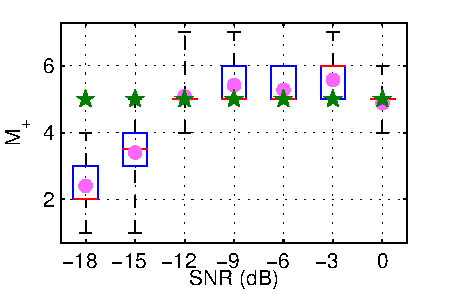
\includegraphics[width=.25\textwidth]{experiments/BoxM_SNR_s.pdf}}
\subfloat[ADER.]{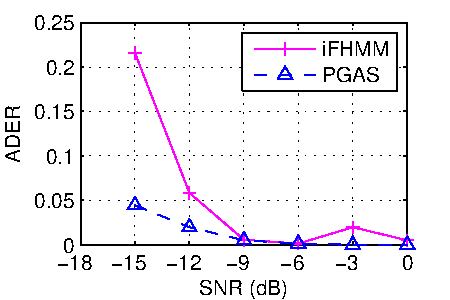
\includegraphics[width=.25\textwidth]{experiments/ADER_SNR_s.pdf}}
\subfloat[SER.]{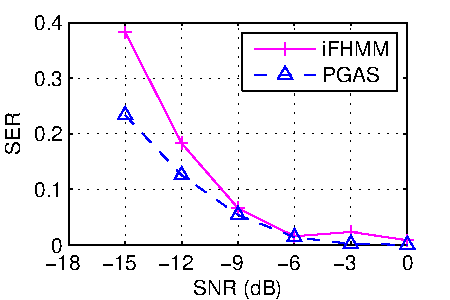
\includegraphics[width=.25\textwidth]{experiments/SER_SNR_s.pdf}}
\subfloat[MSE.]{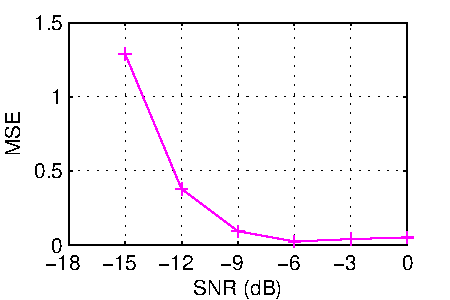
\includegraphics[width=.25\textwidth]{experiments/MSE_SNR_s.pdf}}
\vspace*{-3mm}
\caption{Results for different SNR's.}\label{fig:resultsSNR}
\vspace*{-4mm}
\end{figure*}
%
\begin{figure*}[th]
\centering
\subfloat[Inferred $\hat{M}_+$.]{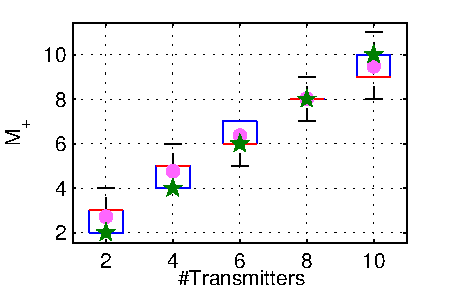
\includegraphics[width=.25\textwidth]{experiments/BoxM_Nt_s.pdf}}
\subfloat[ADER.]{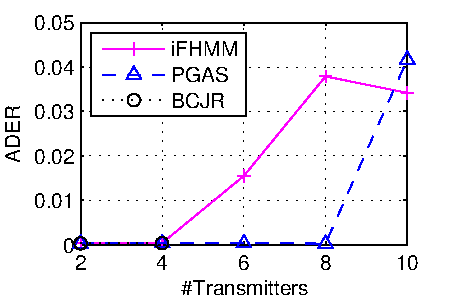
\includegraphics[width=.25\textwidth]{experiments/ADER_Nt_s.pdf}}
\subfloat[SER.]{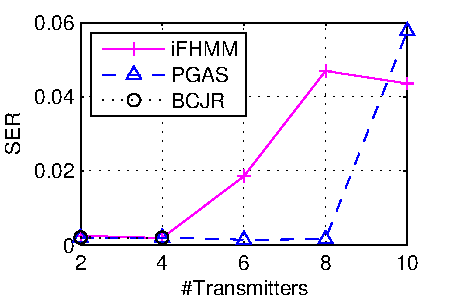
\includegraphics[width=.25\textwidth]{experiments/SER_Nt_s.pdf}}
\subfloat[MSE.]{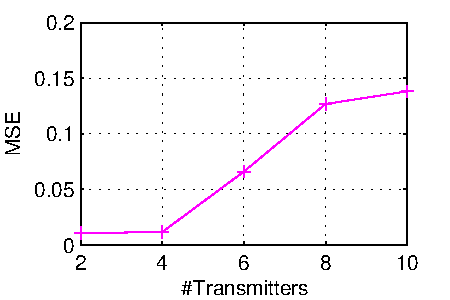
\includegraphics[width=.25\textwidth]{experiments/MSE_Nt_s.pdf}}
\vspace*{-3mm}
\caption{Results for different number of transmitters.}\label{fig:resultsNt}
\vspace*{-4mm}
\end{figure*}

For each considered scenario, we run $50$ independent simulations, each with different simulated data. We run $10,000$ iterations of our inference algorithm described in Section~\ref{sec:inference}, finally obtaining the inferred symbols $\hat{x}_{tm}$ as the component-wise \textit{maximum a posteriori} (MAP) solution, only considering the last $2,000$ iterations of the sampler. The estimates of the channel coefficients $\hathm$ are then obtained as the MAP solution, conditioned on the data and the inferred symbols $\hat{x}_{tm}$. For the BCJR algorithm, we obtain the symbol estimates according to the component-wise MAP solution for each transmitter $m$ and each instant $t$. For the genie-aided PGAS method, we follow a similar approach, considering the last $2,000$ iterations to obtain the symbol estimates.

We choose the following parameters to run our experiments: $M_+=5$ transmitters, $R=20$ receiving antennas, $|\Acal|=4$ symbols in the constellation, and $\textrm{SNR}=-3$~dB. Using this base configuration, we vary one of the parameters while holding the rest fixed.

Figure~\ref{fig:resultsSNR} shows the results when the SNR varies from $-18$~dB ($\sigma_n^2\approx 63.1$) to $0$~dB ($\sigma_n^2=1$). Specifically, we show the ADER, the SER, the MSE, and also the box-plot representation\footnote{We depict the 25-th, 50-th and 75-th percentiles in the standard format, as well as the most extreme values. Moreover, the mean value is represented with a pink circle, and the true number of transmitters $M_+$ is represented with a green star.} of the inferred number of transmitters $\hat{M}_+$. As expected, we obtain a better performance as the SNR increases. For low values of SNR, transmitters are more likely to be masked by the noise and, therefore, we tend to underestimate the number of transmitters. We also observe that, as the SNR increases, the performance (in terms of ADER and SER) of the proposed iFHMM reaches similar values to the PGAS with perfect knowledge of the number of transmitters and channel coefficients.

Figure~\ref{fig:resultsNt} shows the results when the true number of transmitters $M_+$ changes from 2 to 10. As expected, the performance degrades as $M_+$ increases, as more parameters need to be estimated. Nevertheless, we can observe that the iFHMM still tends to recover the true number of transmitters. When the numbers of transmitters becomes larger, we also need larger bursts of transmitted data in order to better estimate the channel coefficients and to reach similar values of the ADER and SER than the genie-aided PGAS.

Figure~\ref{fig:resultsNr} shows the results when the number of receiving antennas varies from 5 to 20. In this figure, we observe that, although our algorithm tends to properly recover the true number of transmitters for any number of receiving antennas, its performance, in terms of ADER and SER, improves when the number of receiving antennas increases, as the diversity in the observations helps to recover the transmitted symbols and channel coefficients. This behaviour is similar to the obtained by the genie-aided PGAS, as shown in this figure.

We show in Figure~\ref{fig:resultsM} the results when the constellation order $|\Acal|$ is changed, ranging from a 4-QAM constellation (also known as QPSK) to a 128-QAM constellation. We can observe that the performance is approximately constant across the considered interval, except in terms of the SER. This makes sense, as increasing the constellation order makes the constellation more dense (we recall that the constellation is normalized in all cases to have unit energy), so it becomes easier to commit an error when estimating each symbol.
%
\begin{figure*}[th]
\centering
\subfloat[Inferred $\hat{M}_+$.]{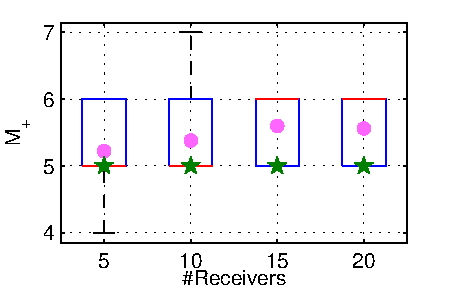
\includegraphics[width=.25\textwidth]{experiments/BoxM_Nr_s.pdf}}
\subfloat[ADER.]{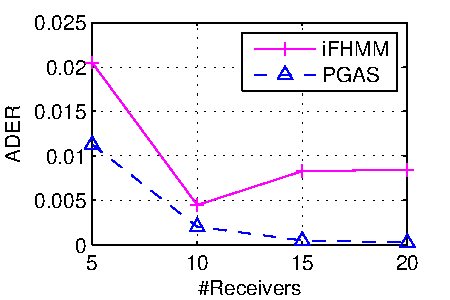
\includegraphics[width=.25\textwidth]{experiments/ADER_Nr_s.pdf}}
\subfloat[SER.]{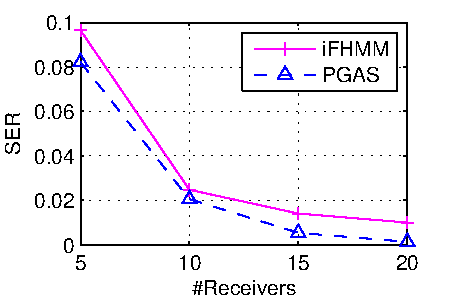
\includegraphics[width=.25\textwidth]{experiments/SER_Nr_s.pdf}}
\subfloat[MSE.]{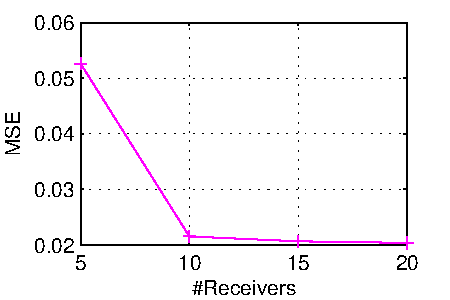
\includegraphics[width=.25\textwidth]{experiments/MSE_Nr_s.pdf}}
\vspace*{-3mm}
\caption{Results for different number of receiving antennas.}\label{fig:resultsNr}
\vspace*{-4mm}
\end{figure*}
%
\begin{figure*}[th]
\centering
\subfloat[Inferred $\hat{M}_+$.]{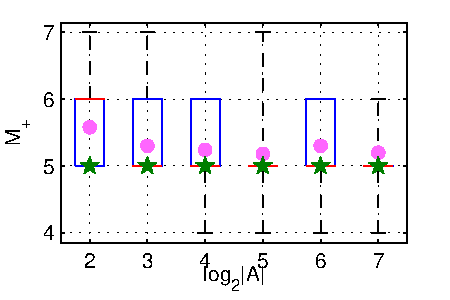
\includegraphics[width=.25\textwidth]{experiments/BoxM_M_s.pdf}}
\subfloat[ADER.]{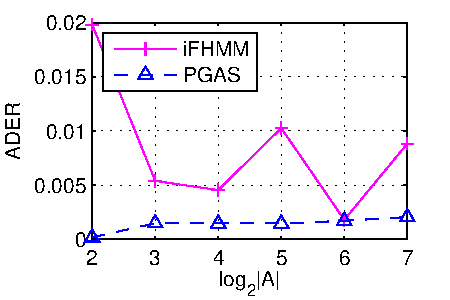
\includegraphics[width=.25\textwidth]{experiments/ADER_M_s.pdf}}
\subfloat[SER.]{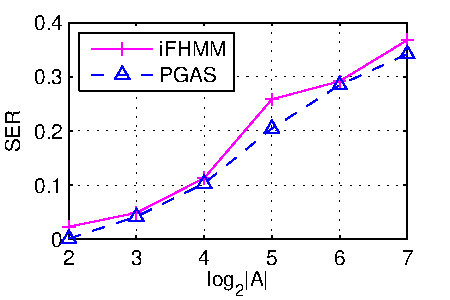
\includegraphics[width=.25\textwidth]{experiments/SER_M_s.pdf}}
\subfloat[MSE.]{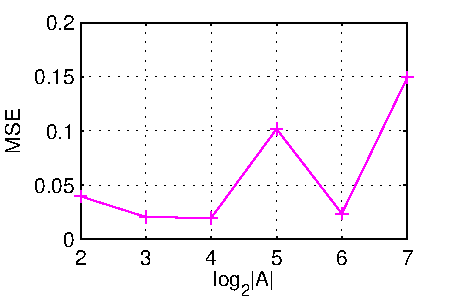
\includegraphics[width=.25\textwidth]{experiments/MSE_M_s.pdf}}
\vspace*{-3mm}
\caption{Results for different constellation order.}\label{fig:resultsM}
\vspace*{-4mm}
\end{figure*}

\section{Conclusions}
\label{sec:conclusions}
We have proposed a fully blind approach for joint channel estimation and detection of the transmitted data when the number of transmitters is unknown. Our approach is based on a BNP model (the iFHMM), for which we have derived an efficient inference algorithm that exploits the properties of MCMC and sequential Monter Carlo techniques. Our experiments on different communication scenarios show that the proposed approach efficiently solves the problem of joint user identification, channel estimation and data detection in a fully blind way.
%
These results are promising for the suitability of BNPs applied to signal processing for communications. However, there is still a lot of work to do in this area. Further research lines may focus on the adaptation of this model to frequency-selective channels, or on improving the scalability of the inference algorithm to account for both a larger number of transmitters and larger observation sequences.  




% References should be produced using the bibtex program from suitable
% BiBTeX files (here: strings, refs, manuals). The IEEEbib.bst bibliography
% style file from IEEE produces unsorted bibliography list.
% -------------------------------------------------------------------------
\bibliographystyle{IEEEbib}
\bibliography{Bib}

\end{document}
